%%%%%%%%%%%%%%%%%%%%%%%%%%%%%%%%%%%%%%%%%%%%%%%%%%%%%%%%%%%%%%%%%%%%%%%%%%%%
% AGUJournalTemplate.tex: this template file is for articles formatted with LaTeX
%
% This file includes commands and instructions
% given in the order necessary to produce a final output that will
% satisfy AGU requirements, including customized APA reference formatting.
%
% You may copy this file and give it your
% article name, and enter your text.
%
%
% Step 1: Set the \documentclass
%
%

%% To submit your paper:
\documentclass[draft]{agujournal2019}
\usepackage{url} %this package should fix any errors with URLs in refs.
\usepackage{lineno}
\usepackage[inline]{trackchanges} %for better track changes. finalnew option will compile document with changes incorporated.
\usepackage{soul}
\linenumbers
\usepackage{graphicx}
\usepackage{amsmath,amsfonts,amsthm,bm}
\DeclareMathOperator{\tr}{tr}
\usepackage{amssymb}
\usepackage[fleqn,tbtags]{mathtools}
\usepackage{siunitx}
\usepackage{multirow}
\usepackage{xcolor}

\renewcommand{\Re}{\operatorname{Re} } 
\renewcommand{\Im}{\operatorname{Im} } 

\linespread{1.6}
%%%%%%%
% As of 2018 we recommend use of the TrackChanges package to mark revisions.
% The trackchanges package adds five new LaTeX commands:
%
%  \note[editor]{The note}
%  \annote[editor]{Text to annotate}{The note}
%  \add[editor]{Text to add}
%  \remove[editor]{Text to remove}
%  \change[editor]{Text to remove}{Text to add}
%
% complete documentation is here: http://trackchanges.sourceforge.net/
%%%%%%%

\draftfalse

%% Enter journal name below.
%% Choose from this list of Journals:
%
% JGR: Atmospheres
% JGR: Biogeosciences
% JGR: Earth Surface
% JGR: Oceans
% JGR: Planets
% JGR: Solid Earth
% JGR: Space Physics
% Global Biogeochemical Cycles
% Geophysical Research Letters
% Paleoceanography and Paleoclimatology
% Radio Science
% Reviews of Geophysics
% Tectonics
% Space Weather
% Water Resources Research
% Geochemistry, Geophysics, Geosystems
% Journal of Advances in Modeling Earth Systems (JAMES)
% Earth's Future
% Earth and Space Science
% Geohealth
%
% ie, \journalname{Water Resources Research}

\journalname{JGR: Solid Earth}


\begin{document}

%% ------------------------------------------------------------------------ %%
%  Title
%
% (A title should be specific, informative, and brief. Use
% abbreviations only if they are defined in the abstract. Titles that
% start with general keywords then specific terms are optimized in
% searches)
%
%% ------------------------------------------------------------------------ %%

% Example: \title{This is a test title}

\title{Poroelastic effects of secondary fractures on fracture reflectivity }

%% ------------------------------------------------------------------------ %%
%
%  AUTHORS AND AFFILIATIONS
%
%% ------------------------------------------------------------------------ %%

% Authors are individuals who have significantly contributed to the
% research and preparation of the article. Group authors are allowed, if
% each author in the group is separately identified in an appendix.)

% List authors by first name or initial followed by last name and
% separated by commas. Use \affil{} to number affiliations, and
% \thanks{} for author notes.
% Additional author notes should be indicated with \thanks{} (for
% example, for current addresses).

% Example: \authors{A. B. Author\affil{1}\thanks{Current address, Antartica}, B. C. Author\affil{2,3}, and D. E.
% Author\affil{3,4}\thanks{Also funded by Monsanto.}}

\authors{Edith Sotelo\affil{1}, J. Germ\'{a}n Rubino\affil{2},  Nicol\'{a}s D. Barbosa\affil{1}, Santiago G. Solazzi\affil{1}, Klaus Holliger\affil{1}}


% \affiliation{1}{First Affiliation}
% \affiliation{2}{Second Affiliation}
% \affiliation{3}{Third Affiliation}
% \affiliation{4}{Fourth Affiliation}

 \affiliation{1}{Institute of Earth Sciences, University of Lausanne, Lausanne, Switzerland }
 \affiliation{2}{CONICET, Centro Atómico Bariloche - CNEA, San Carlos de Bariloche, Argentina}
%(repeat as many times as is necessary)

%% Corresponding Author:
% Corresponding author mailing address and e-mail address:

% (include name and email addresses of the corresponding author.  More
% than one corresponding author is allowed in this LaTeX file and for
% publication; but only one corresponding author is allowed in our
% editorial system.)

% Example: \correspondingauthor{First and Last Name}{email@address.edu}

\correspondingauthor{Edith Sotelo}{edith.sotelogamboa@unil.ch}

%% Keypoints, final entry on title page.

%  List up to three key points (at least one is required)
%  Key Points summarize the main points and conclusions of the article
%  Each must be 140 characters or fewer with no special characters or punctuation and must be complete sentences

% Example:
% \begin{keypoints}
% \item	List up to three key points (at least one is required)
% \item	Key Points summarize the main points and conclusions of the article
% \item	Each must be 140 characters or fewer with no special characters or punctuation and must be complete sentences
% \end{keypoints}

\begin{keypoints}
\item enter point 1 here
\item enter point 2 here
\item enter point 3 here
\end{keypoints}

%% ------------------------------------------------------------------------ %%
%
%  ABSTRACT and PLAIN LANGUAGE SUMMARY
%
% A good Abstract will begin with a short description of the problem
% being addressed, briefly describe the new data or analyses, then
% briefly states the main conclusion(s) and how they are supported and
% uncertainties.

% The Plain Language Summary should be written for a broad audience,
% including journalists and the science-interested public, that will not have 
% a background in your field.
%
% A Plain Language Summary is required in GRL, JGR: Planets, JGR: Biogeosciences,
% JGR: Oceans, G-Cubed, Reviews of Geophysics, and JAMES.
% see http://sharingscience.agu.org/creating-plain-language-summary/)
%
%% ------------------------------------------------------------------------ %%

%% \begin{abstract} starts the second page

\begin{abstract}
Abstract
\end{abstract}

\section*{Plain Language Summary}
Plain language summary


%% ------------------------------------------------------------------------ %%
%
%  TEXT
%
%% ------------------------------------------------------------------------ %%

%%% Suggested section heads:
% \section{Introduction}
%
% The main text should start with an introduction. Except for short
% manuscripts (such as comments and replies), the text should be divided
% into sections, each with its own heading.

% Headings should be sentence fragments and do not begin with a
% lowercase letter or number. Examples of good headings are:

% \section{Materials and Methods}
% Here is text on Materials and Methods.
%
% \subsection{A descriptive heading about methods}
% More about Methods.
%
% \section{Data} (Or section title might be a descriptive heading about data)
%
% \section{Results} (Or section title might be a descriptive heading about the
% results)
%
% \section{Conclusions}


\section{Introduction}

\section{Theory and methods}
We consider a model in $\mathbb R^2$ comprised of a poroelastic fracture system embedded in a  background deemed impermeable for the frequencies of interest (Figure \ref{fig.1}). The fracture system consists of an infinite main horizontal fracture that is intersected by equally spaced vertical secondary fractures.

We take a two-step approach
to investigate the poroelastic effects that intersecting secondary fractures induce on a main  fracture reflectivity at normal incidence. In the first step, we quantify the effective viscoelastic P-wave modulus and the associated viscoelastic compliance of the main that results from the fracture to fracture FPD.

 To this end, we apply the  poro-to-viscoelastic homogenization procedure as proposed by cite() on 2D models similar to Figure (fig xx). This figure shows a sample $\Omega$ consisting of a main horizontal poroelastic fracture that is normally intersected by a secondary one that is also poroelastic. This fracture system is embedded in impermeable background. Then, for the reflectivity analysis, we consider simplified 1D models similar to Figure (figure xx) that only include the main fracture embedded in the  impermeable background, where the former is represented by a viscoelastic medium after the poro-to-viscoelastic homogenization. We disregard the effect of the secondary fractures because the mechanical and poroelastic impact of fractures parallel to the traveling P-wave can be deemed negligible. (fix this)

In the following, we describe in further detail these aforementioned steps.


\subsection{Homogenization procedure}

\subsubsection{Mesoscale fluid pressure diffusion}

 \begin{figure}[!ht]
\centering
        \includegraphics[ width= 100mm, height=80mm]{fracture_system.eps}
\caption{
}
\label{fig.1}
\end{figure}
We assume an incoming P-wave striking normally to the main fracture as shown  in figure \ref{fig.1}. This wave produces an increment of the pore pressure in the main fracture, which, in turn, equilibrates by inducing fluid flow towards the secondary fractures. For sufficient low frequencies, which are in general within the fracture frequency range, this fracture-to-fracture wave-induced fluid flow is driven by fluid pressure diffusion (FPD) \cite{Muller2010}.
We are interested in FPD that occurs at mesoscale heterogeneities since this is particular relevant for seismic applications \cite{Pride2004, Muller2010}.
Mesoscale heterogeneities refer to those with characteristic length-scales  $L_h$ larger than the pore scale $L_p$ but smaller than the wavelength $\lambda_w$. For the considered fracture system, the mesoscale heterogeneities are dictated by the characteristic sizes of the fractures, for instance, the length of the secondary fractures \cite{Rubino2014}.
On the other hand, this FPD  mechanism is constrained to frequencies $f$ that are much lower than Biot's characteristic frequency $f_B$  \cite{Biot1956, Dutta1979}
\begin{linenomath*}
\begin{equation}\label{Eq.1}
f_B= \frac{1}{2 \pi} \frac{\eta \phi}{ \rho_f \kappa S },
\end{equation}
\end{linenomath*}
where $\phi$ is the porosity, $\kappa$  the static permeability, $\eta$, the fluid viscosity,  $\rho_f$ the fluid density, and $S$ the tortuosity of the pore space. The aformentioned considerations regarding frequencies and scales constraining mesoscale FPD can be summarized as
\begin{linenomath*}
\begin{equation}\label{Eq.2}
\begin{split}
f & \ll f_B\\
L_p & \ll L_h\ll \lambda_w.
\end{split}
\end{equation}
\end{linenomath*}

It can be shown that the diffusion coefficient $D$ and the characteristic diffusion $L_d$ associated with FPD are \cite{Chandler1981, Norris1993}
\begin{linenomath*}
\begin{equation}\label{Eq.3}
\begin{split}
&L_d=\sqrt{\frac{D}{\omega}},\quad \text{with} \\
&D= \frac {\kappa} {\eta} \frac{M H_d}{H},
 \quad \text{and}  
\end{split}
\end{equation}
\end{linenomath*}
where $M$ is Biot’s fluid storage modulus, $H_d$ and $H$ are the drained and undrained plane-wave moduli, respectively, and $\omega$ is the angular frequency $\omega = 2 \pi f$.        
The required rock physical properties are calculated as
\begin{linenomath*}
\begin{equation}\label{Eq.4}
\begin{split}
& H_d = \lambda_d + 2 \mu, \\
& H = H_d + M \alpha ^2, \\
& \lambda_d= K_m - \frac{2}{3} \mu, \\
& \alpha =1-\frac{K_m}{K_s},\\
& M  =\left( \frac{\alpha-\phi}{K_s} +\frac{\phi}{K_f} \right)^{-1},
\end{split}
\end{equation}
\end{linenomath*}
where $\lambda_d$ is the the drained Lamé modulus, $\mu$ is the shear modulus, $\alpha$ is the Biot-Willis effective stress coefficient, $K_m$, $K_s$, and $K_f$ are the bulk moduli of the drained solid frame, the solid grains, and the pore fluid, respectively.

On the other hand, FPD is characterized by two limiting regimes, the relaxed and unrelaxed states, that are controlled by the wave-frequency, the characteristic diffusion length $L_d$ and the characteristic size of the heterogeneities $L_f$ 
The relaxed state occurs at sufficiently low frequencies, for which  $L_d \gg L_h$. In this regime, there is enough time for the pressure between the main and secondary fractures to equilibrate. Conversely, the unrelaxed state occurs at sufficiently high frequencies, for which $L_d \ll L_h$ and, consequently, there is insufficient time for pressure equilibration to take place and, hence, the main and secondary fractures are hydraulically isolated. A transition zone exists at intermediate frequencies for which $L_d \approx L_h$ that is associated with attenuation and dispersion of body waves due to viscous dissipation. The maximum dissipation of energy is associated with a maximum a characteristic transition frequency $f_c= \omega_c/2\pi$, 
which depends on the diffusion coefficient $D$ and the characteristic size of the heterogeneity $L_h$ \cite{Rubino2014}
\begin{linenomath*}
\begin{equation}\label{Eq.5}
\omega_c \propto \frac{D}{(L_h)^2}.
\end{equation}
\end{linenomath*}

The described FPD relaxation mechanism produces a viscoelastic behavior of the main fracture P-wave modulus and, consequently, of its normal compliance. 
The frequency-dependent P-wave modulus of the  main fracture ca be estimated by solving \citeauthor{Biot1941}'s \citeyear{Biot1941} on a representative sample of the fractured model of Figure \ref{fig.1}, while applying a vertical compressional oscillatory test. This is 
followed by the volume averaging of the vertical strain and stress components, which are then used to estimate the frequency dependent P-wave modulus. On the other hand, the viscoelastic characteric of the P-wave modulus due to FPD produces attenuation and dispersion of the associated P-wave, where the maximum attenuation occurs at the characteristic transition frequency $f_c$.


\subsubsection{Governing equations}

 \begin{figure}[!ht]
\centering
        \includegraphics[ width= 80mm, height=80mm]{2fracture.eps}
\caption{
}
\label{fig.2}
\end{figure}
We solve Biot's consolidation equations \cite{Biot1941} over the sample $\Omega$  for the vertical compressional oscillatory relaxation test as detailed in Equations
\eqref{Eq.8} and \eqref{Eq.9}. 
We express these equations in the solid displacement - pressure ($\bm{u}-p$) formulation in the frequency domain \cite{Quintal2011,Favino2020},  with $\bm{u} = \bm{u}(\bm{x}, \omega)$ and $p = p(\bm{x},\omega)$, where $\bm{x} \in \Omega$ is the position  and $\omega \in F$ is the angular frequency, with $F =(0,W]$. 
\begin{linenomath*}
\begin{equation}\label{Eq.6}
\begin{split}
& - \nabla \cdot \, \bm{\sigma} =0  \quad  \textrm{in} \quad \Omega \times F,  \\
& - i \, \alpha \nabla . \, \bm{u} -i \frac{p}{M} + \frac{1}{\omega} \,\nabla \, \cdot \, \left( \frac{\kappa}{\eta} \nabla p\right)  =0 \quad  \textrm{in} \quad \Omega \times F,
\end{split}
\end{equation}
\end{linenomath*}
where $\bm{\sigma}$ is the total stress and $i$ is the imaginary unit.

The constitutive equation relating the total stress $\bm{\sigma}$ to $\bm{u}$ and $p$ is
\begin{linenomath*}
\begin{equation}\label{Eq.7}
\begin{split}
& \bm{\sigma} =  2\mu \, \bm{\varepsilon} +  \left( \lambda_d \,  \tr( \bm{\varepsilon})\, - \alpha \,p \right) \bm{I}, \qquad \text{with}\\
& \bm{\varepsilon} = \frac{1}{2} \left( \nabla \,\bm{u} + ({\nabla  \bm{u}})^T  \right),
\end{split}
\end{equation}
\end{linenomath*}
where $\bm{\varepsilon}$ is the strain tensor and $\bm{I}$ the identity tensor. 


\subsubsection{Vertical compressional oscillatory relaxation test}
In this subsection, we detail the BC for the vertical oscillatory relaxation test. We assume a Cartesian coordinate system in $\mathbb R^2$ with the associated basis vectors $\bm{\hat x_1}$ and $\bm{\hat x_3}$ parallel to the horizontal and vertical Cartesian axes, respectively. We also
let the sample $\Omega$ be a quadrilateral with boundary $\Gamma = \Gamma_1^+ \cup \Gamma_1^- \cup \Gamma_3^+ \cup \Gamma_3^- $, where $\Gamma_1^+ $ and $\Gamma_1^- $ are opposite boundaries with outer normal vectors $\bm{\hat x_1}$ and $ -\bm{\hat x_1}$, respectively. Similarly, $\Gamma_3^+ $ and $\Gamma_3^- $ are opposite boundaries with outer normal vectors $\bm{\hat x_3}$ and $ -\bm{\hat x_3}$ (Figure \ref{fig.2}). To simplify the notation, we let $ \bm{\hat n}$ be the outer normal vector
of $\Gamma$.

In the following, define the BC for displacements, pressure, tractions and fluid flux relative to the solid, imposing periodicity to the respective variables on opposite boundaries. 
The BC for displacements are

\begin{linenomath*}
\begin{equation}\label{Eq.8}
\begin{split}
&  \bm{u} \cdot \bm{\hat{x}_3} \, \vert_{\Gamma_3^-} - \bm{u}\cdot \bm{\hat{x}_3}\, \vert_{\Gamma_3^+} =- \Delta u, \\
&  \bm{u} \cdot \bm{\hat{x}_1}\, \vert_{\Gamma_3^-} - \bm{u} \cdot \bm{\hat{x}_1} \, \vert_{\Gamma_3^+} = 0, \\
& \bm{u}\,\vert_{\Gamma_1^+} - \bm{u}\,\vert_{\Gamma_1^-} = \bm{0},
\end{split}
\end{equation}
\end{linenomath*}
where $\Delta u$ is a real displacement difference in the frequency domain.

The respective BC for pressure, tractions and fluid flux relative to the solid are
\begin{linenomath*}
\begin{equation}\label{Eq.9}
\begin{split}
& p\vert_{\Gamma_k^+}-p\vert_{\Gamma_k^-} =0, \\
& \left(\bm{\sigma}\cdot \bm{\hat n} \right)\, \vert_{\Gamma_k^+}-\left(\bm{\sigma}\cdot \bm{\hat n} \right)\, \vert_{\Gamma_k^-} = \bm{0},\\
&\left( \frac{\kappa}{\eta} \nabla p \cdot \bm{\hat n} \right) \, \vert_{\Gamma_k^+} -\left( \frac{\kappa}{\eta} \nabla p \cdot \bm{\hat n} \right) \, \vert_{\Gamma_k^-} = 0,
\end{split}
\end{equation}
\end{linenomath*}
where the subscript $k$ in $\Gamma_k^-$ and $\Gamma_k^+$ takes the value of 1 or 3 at a time to denote opposite boundaries.

\subsubsection{Plane-wave modulus}

Here, we detail the calculations to obtain the plane-wave modulus and normal compliance of the main horizontal fracture.  To this end, we first take the average of  of the stress component $\langle \sigma_{33} \rangle_{\Omega_{p1}}$ and of the respective strain component $\langle \varepsilon_{33} \rangle_{\Omega_{p1}}$ only over $\Omega_{p1}$ (Figure \ref{fig.2}). The corresponding average quantities $\langle \Box \rangle_{\Omega_{p1}}$ are computed as
\begin{linenomath*}
\begin{equation}\label{Eq.10}
\begin{split}
&\langle \Box \rangle_{\Omega_{p1}} = \frac{1}{\vert \Omega_{p1} \vert} \int_{\Omega_{p1}} \Box \, d\Omega_{p1}, \qquad \text{with} \quad  \vert \Omega_{p1} \vert = \int_{\Omega_{p1}}  d\Omega_{p1}.
\end{split}
\end{equation}
\end{linenomath*}

Then, we calculate the main P-wave plane modulus as
\begin{linenomath*}
\begin{equation}\label{Eq.11}
H(\omega)= \frac{\langle \sigma_{33} \rangle_{\Omega_{p1}}}{\langle \varepsilon_{33} \rangle_{\Omega_{p1}}}.
\end{equation}
\end{linenomath*} 

Finally, we obtain the main fracture normal compliance $Z_N (\omega) $ as
\begin{linenomath*}
\begin{equation}\label{Eq.12}
Z_N(\omega)= \frac{a_f}{H(\omega)}, 
\end{equation}
\end{linenomath*} 
where $a_f$ is the aperture of the main fracture.

On the other hand, the inverse of the P-wave attenuation coefficient $Q_P^{-1}$ is also related to the P-wave modulus and, as previously stated, its maximum value $max\, Q_P^{-1} $ occurs at the characteristic transition frequency $f_c$, which is associated with maximum energy dissipation. We express $Q_P^{-1}$ as
\begin{linenomath*}
\begin{equation}\label{Eq.13}
Q_P^{-1}= \frac{\Im(1/H(\omega))}{\Re(1/H(\omega))}, 
\end{equation}
\end{linenomath*} 

\subsection{Normal reflectivity of the main fracture}

We consider a simplified  model in as shown in Figure \ref{fig.3}. In this model, the main fracture is represented by a viscoelastic layer $\Omega_v$ and is embedded in the same  half-spaces $\Lambda_1$ and $\Lambda_2$, respectively (Figure \ref{fig.1}).
We also consider an incoming P-wave striking normally at the interface $\Pi_1$ between the upper half-space and the fracture. In the following, we detail the procedure to find the PP reflection coefficients $R_{PP}$ at this interface.

 \begin{figure}[!ht]
\centering
        \includegraphics[ width= 80mm, height=80mm]{mainfracture.eps}
\caption{
}
\label{fig.3}
\end{figure}

\subsubsection{Governing equations}
We formulate the elastic and viscoelastic wave equations in the space-frequency domain. 

For the elastic wave equation, we let $\bm{u}^e=\bm{u}^e (\bm{x},\omega)$ be the displacement vector for any position $\bm{x}$ $\in n$, with  $n= \{\Lambda_1, \Lambda_2\} $ and angular frequency  $\omega \in F$ , with $F =(0,W]$. We also let $\bm{\sigma}^e$ be the stress tensor field acting upon the medium. Then, we express the corresponding equation of motion as
\begin{linenomath*}
\begin{equation}\label{Eq.14}
- \, \rho_b \,\omega^2 \, \bm{u}^e = \nabla . \, \bm{\sigma}^e \quad  \textrm{in} \quad n \times F.
\end{equation}
\end{linenomath*}
The associated constitutive equation is given by: 
\begin{linenomath*}
\begin{equation}\label{Eq.15}
\bm{\sigma}^e = \mu \,  \left( \nabla \, \bm{u}^e + ({\nabla  \bm{u}^e})^T  \right) + \lambda \,  \nabla . \, \bm{u}^e\,\, \bm{I},
\end{equation}
\end{linenomath*}
where $\lambda$ is the undrained Lamé modulus and is calculated as $\lambda = \lambda_d + M \alpha^2$.

For the viscoelastic wave equation, we let $\bm{u}^v=\bm{u}^v (\bm{x},\omega)$ be the displacement vector for any position $\bm{x}$  $ \in \Omega_v$ and angular frequency $\omega \in F$ , with $F =(0,W]$. We also let $\bm{\sigma}^v$ be the stress tensor field acting upon the medium. Then, we express the corresponding equation of motion as:
\begin{linenomath*}
\begin{equation}\label{Eq.16}
- \, \rho_b \,\omega \, \bm{u}^v = \nabla . \, \bm{\sigma}^v \quad \textrm{in} \quad \Omega_v \times F.
\end{equation}
\end{linenomath*}
The associated constitutive equation is given by: 
\begin{linenomath*}
\begin{equation}\label{Eq.17}
\begin{split}
& \bm{\sigma}^v = \mu \,  \left( \nabla \, \bm{u}^v + ({\nabla  \bm{u}^v})^T  \right) + \lambda(\omega) \,  \nabla . \, \bm{u}^v\,\, \bm{I}, \quad \text{with} \\
& \lambda(\omega)= H(\omega)-2\mu.
\end{split}
\end{equation}
\end{linenomath*}

\subsubsection{Solution for displacements}
As stated, we assume an incoming P-wave strikes normally the interface $\Pi_1$  between the upper half-space and the fracture (Figure \ref{fig.3}), which are represented by elastic and poroelastic media, respectively. As a consequence, only P-waves propagate vertically in both half-spaces and in the fracture. Then, to find the total displacement in each medium we sum the corresponding ones produced by the upgoing and downgoing P-wave, respectively.

For the elastic half-spaces $n =\{\Lambda_2, \Lambda_2\}$, we let $u_n^e$ be the corresponding total displacements, which are calculated as
\begin{linenomath*}
\begin{equation}\label{Eq.18}
\begin{split}
& u_n^e=  u_{n\,{D_P}}^e + u_{n\,{U_P}}^e \quad \text{when}\, n=\Lambda_1 , \, \text{or}  \\
& u_n^e = u_{n\,{D_P}}^e \quad \text{when}\, n=\Lambda_2 ,
\end{split}
\end{equation}
\end{linenomath*}
where $D$ and $U$ refer to the downgoing and upgoing waves, respectively, and the subscript $P$ refers to the P-wave.
% Since in the lower half-space $\Lambda_2$ there are no upgoing P-wave, $u_n^e$ simplifies to:
%\begin{linenomath*}
%\begin{equation}\label{Eq.18}
%u_n^e = u_{n\,{D_P}}^e.
%\end{equation}
%\end{linenomath*}

Then, we express the corresponding solution $u_{n\,j}^e$ for each elastic medium $n$ = $\Lambda_1$ and $\Lambda_2$, with $j$ = $D_P$ or $U_P$, as
\begin{linenomath*}
\begin{equation}\label{Eq.19}
u_{n\,j}^e = E_{n \,j} \;\exp[ \pm\; i \; k_{n}^e \; x_3 ]\,,
\end{equation}
\end{linenomath*}
where $E_{n \,j}$ is the amplitude of the corresponding elastic displacement and $x_3$ is the position. Negative and positive signs in the exponential correspond to downgoing and upgoing waves, respectively, $ k_{n}^e$ is the elastic scalar wavenumber for the P-wave in medium $n$, calculated as $ k_{n}^e$ = $\omega / V_P^n$, where $V_P^n$ is the P-wave velocity of medium $n$, with $V_P^n = \sqrt{(\lambda^n +  2\, \mu^n)/\rho_b^n}$
%The corresponding $V_P^n$ is
%\begin{linenomath*}
%\begin{equation}\label{Eq.20}
%V_P^n = \sqrt{\frac{\lambda^n +  2\, \mu^n}{\rho_b^n}}.
%\end{equation}
%\end{linenomath*}

For the viscoelastic medium $\Omega_v$, we let  $u^v$ be the total viscoelastic displacement given by 
\begin{linenomath*}
\begin{equation}\label{Eq.20}
u^v=  u_{\,D_P}^v  + u_{\,U_P}^v.
\end{equation}
\end{linenomath*}

Then, we express the solution of the corresponding displacement $u_j^v$, with $j = D_P , U_P$ as
\begin{linenomath*}
\begin{equation}\label{Eq.21}
u_j^v = V_j \;\exp[ \pm\; i \; k^v \; x_3 ]\,,
\end{equation}
\end{linenomath*}
where $V_j$ is the amplitude of the corresponding viscoelastic displacement, $ k^v$ is the viscoelastic scalar wavenumber for the P-wave calculated as $ k^v=\omega / V_P(\omega)$, where $V_P(\omega)$ is the frequency-dependent P-wave velocity that is computed as $V_P(\omega) = \sqrt{H(\omega) /\rho_b }$
%\begin{linenomath*}
%\begin{equation}\label{Eq.23}
%V_P(\omega) = \sqrt{ \frac{H(\omega) }{\rho_b} }.
%\end{equation}
%\end{linenomath*}

\subsubsection{PP reflection coefficients}
We assume that the amplitude of the incident P-wave is one, then the reflection coefficient $R_{PP}$ at the upper half-space is equal to $E_{\Lambda_1\, UP}$ (Equation \eqref{Eq.18}). To solve for the unknown amplitudes,  we assemble a set of equations by imposing continuity of displacements and tractions at the elastic-viscoelastic interfaces $\Pi_q$, respectively, with $q=1,2$
\begin{linenomath*}
\begin{equation}\label{Eq.22}
\begin{split}
&  \left. \left(  u_n^e -  u^v \right) \right \rvert_{\Pi_q} = 0 \,, \\
&  \left. \left( t_n^e  - t^v  \right) \right \rvert_{\Pi_q} = 0 \,.
\end{split}
\end{equation}
\end{linenomath*}
Here, $n$ = $\Lambda_q$, $t_n^e$ and $t^v$ are the normal traction components on the elastic and viscoelastic sides of the interface, respectively. They are calculated as $t_n^e =( \bm{\sigma_n}^e \cdot \bm{\hat {x}_3})\cdot \bm{\hat {x}_3} $ and  
$t^v =( \bm{\sigma}^v \cdot \bm{\hat {x}_3})\cdot \bm{\hat {x}_3} $, respectively.

\section{Results}

In the following we present a sensitivity analysis where we vary the geometrical and physical properties of the secondary fractures to investigate their impact on the normal compliance and reflectivity of the main fracture. 
We compare the  results against those obtained using a model that considers only the main fracture embedded in impermeable background. In this model the fracture presents an undrained behavior because it is hydraulically isolated.

Table \ref{table.1} and Table \ref{table.2} show the reference rock and physical properties for the main fracture, secondary fractures, the impermeable half-spaces and the pore fluids, respectively. Unless otherwise stated, we assume that both fractures are water-saturated. Besides, to obtain both the frequency-dependent P-wave modulus and normal compliance of the main fracture for the different tested models,  we apply the homogenization procedure described in the Methodology section using a square sample $\Omega$ (Figure \ref{fig.2}) with a side length of 0.8 m. On the other hand, as previously stated, the poroelastic-to-viscoelastic homogenization is valid for frequencies that are below Biot's characteristic frequency (Equation \eqref{Eq.1}). The corresponding values for the main and secondary fractures are 1.3 KHz and 12.9 KHz, respectively, which are below the seismic frequency range.

\begin{table}[!ht]
  \caption{Reference values of the physical properties for the main fracture, secondary fractures, and the background, respectively (Figure \ref{fig.1}). }
\begin{center}
  \begin{tabular}{ | l c  c  c | }
    \hline
    Property & Main fracture ($f$) & Secondary fracture ($h$) & Background rock \\ \hline
    Grain bulk modulus $K_s$ (GPa) & 37 & 37 & 37 \\ 
    Porosity $\phi$ & 0.8 & 0.8 & 0.015 \\ 
    Frame bulk modulus $K_m$ (GPa) &  0.004 & 0.016 & 37\\ 
    Frame shear modulus $\mu$ (GPa) & 0.002 & 0.008 & 29\\
    Permeability $\kappa$ (D) & 100 & 10 & 1.e-12\\
    Aperture $a$ (m) & 0.001 & 0.001 & NA\\
    Length $L$ (m) & infinite & 0.76 & NA \\
    Spacing $s$ (m) & NA & 0.8 & NA \\
    Grain density $\rho_s$ ($\rm{Kg/m^3}$) & 2730 & NA & 2730\\ 
    \hline
  \end{tabular}
  \label{table.1}
\end{center}
\end{table}

\begin{table}[!ht]
  \caption{Reference values of the physical properties of pore fluids}
\begin{center}
  \begin{tabular}{ | l  c  c |  }
    \hline
    Property & Water & Gas\\ \hline
    Fluid density $\rho_f$ ($\rm{Kg/m^3}$) & 1000 & 78\\
    Fluid bulk modulus $K_f$ (\rm{GPa}) & 2.25 & 0.012\\
    Fluid viscosity $\eta$ (\rm{Pa.s})& 1.e-3 & 1.5e-4\\
    \hline
  \end{tabular}
  \label{table.2}
\end{center}
\end{table}
We present the plots of the frequency-dependent fracture normal compliance $Z_N (\omega)$ as a ratio ($Z_N\, \text{ratio}$) against its undrained value $Z^u_{N}$. This is $Z_N\, \text{ratio}=Z_N (\omega)/ Z^u_{N}$, where the undrained normal compliance  $Z^u_{N}$ designates the minimum value that $Z_N (\omega)$ can take. Using the properties for the main fracture from Table \ref{table.1}, we  find that $Z^u_{N} =3.6 \times 10 ^{-13}$  m/Pa. On the other hand, the drained normal compliance $Z^d_{N}$ denotes maximum value that $Z_N (\omega)$ can take, which we calculate as:
$Z^d_{N}= a_f/H_d$. Using again the properties for the main fracture from Table \ref{table.1}, we find that $Z^d_{N} =1.5\times 10^{-10} $ m/Pa. Then, the maximum value than the ratio $Z_N\, \text{ratio}$  can take happens when  $Z_N (\omega) = Z^d_{N} $, which yields 416.5. Besides,
we estimate the associated characteristic frequency $f_c$ by finding the frequency for which the P-wave attenuation reaches its maximum ($max\, Q_P^{-1}$), where $Q_P^{-1}$ is calculated using Equation \eqref{Eq.13}.


\subsection{Sensitivity to the geometrical properties of the secondary fractures}
In this subsection, we investigate the sensitivity of the main fracture normal compliance and of its reflectivy response to the variation of the geometrical properties of the secondary fractures, such as length $L^h$, aperture $a^h $ and spacing $s^h$, respectively. To perform this sensitivity analysis, we modify one parameter at a time by halving subsequently its value from its reference one as shown in Table \ref{table.1} for a total of an eight-fold decrease.

Figure \ref{fig.4} presents the $Z_N\, \text{ratio}$ as a function of frequency for the different geometrical parameters of the secondary fractures. The results show that there is an increase of the normal compliance of the main fracture with respect to its undrained value ( $Z_N\, \text{ratio}$ =  1) as a consequence of FPD prevailing in regimes other than the unrelaxed one between the main and secondary fractures. In particular, we observe that all curves present a similar behavior with respect to the frequency. This is, at sufficient low frequencies 
%For instance, the maximum  $Z_N\, \text{ratio}$ is 67.5 for the reference properties of the secondary fractures listed in Table \ref{table.1} (e.g., Figure \ref{fig.4}a and curve $L^h$ = 0. 76 m).
$Z_N\, \text{ratio}$ shows a constant maximum as a consequence of FPD prevailing in the relaxed regime. Then, as frequency increases it decreases monotonically towards its undrained value.
Nonetheless, the sensitivity to their different geometrical properties is not the same.
According to the results, the changes in normal compliance of the main fracture is the most sensitive to variations of the length $L^h$ of secondary fractures (Figure \ref{fig.4}a) and is the least sensitive to variations in their spacing $s^h$ (Figure \ref{fig.4}c). An intermediate sensitivity is associated to variations of their aperture $a^h$ (Figure \ref{fig.4}b). Specifically, the maximum $Z_N\, \text{ratio}$ shows a 35.5-fold increase, from 1.9 to 67.5, for the corresponding eight-fold increase in length $L^h$. Then, the maximum  $Z_N\, \text{ratio}$ increases close to four-folds, from 17.5 to 67.5, for a similar aperture $a^h$ increase of eight-fold. Finally, the maximum $Z_N\, \text{ratio}$  presents the lowest increase of 1.7-folds, from 67.5 to 113.4, in response to the eight-fold decrease in spacing $s^h$. On the other hand, the parameters tested impact in different degrees the characteristic transition frequency $f_c$. For instance, $f_c$ shows the highest sensitivity to changes in length $L^h$ of the secondary fractures (Figure \ref{fig.4}a), taking decreasing values from $\sim$ 1.0 KHz to $\sim$ 6.3 Hz as the length $L^h$ increases. In contrast, $f_c$ is the least sensitive to changes in the aperture $a^h$ of the secondary fractures (Figure \ref{fig.4}b). In this case $f_c$, takes increasing values from  $\sim$ 2.5 Hz to  $\sim$ 6.3 Hz as the aperture $a^h$ increases. Finally, $f_c$ presents an intermediate sensitivity to the spacing $s^h$ of the secondary fractures (Figure \ref{fig.4}c), where $f_c$ decreases from  $\sim$ 25.1 Hz to  $\sim$ 6.3 Hz with increasing spacing.

On the other hand, the previously described sensitivity of normal fracture compliance and transition frequency to variations of the geometrical properties has also an impact on the PP reflectivity of the main fracture at normal incidence. In this regard, Figure \ref{fig.5} shows the absolute value of PP as a function of frequency for the same geometrical parameters of the secondary fractures presented in Figure \ref{fig.4}. We observe that for all the cases tested, the PP reflectivity of the main fracture increases from its elastic value as a consequence of FPD occurring between the main and secondary fractures. Specifically, all curves show a similar pattern with respect to frequency. This is, for sufficient low frequencies the reflectivity has a maximum constant increase from the elastic reference as a consequence of FPD occurring in the relaxed regime. Then, as frequency increases, the reflectivity decrease towards the elastic value in response to the prevailing transition FPD regime. Regarding the sensitivity of the main fracture reflectivity to changes in geometrical properties of the secondary fractures, the results show that it presents a similar behavior as the one described for its normal compliance. This is, its reflectivity at normal incidence is the most sensitive to changes in length $L^h$, then aperture $a^h$ and finally to spacing $s^h$. Specifically, the maximum increase of reflectivity is around two orders of magnitude for an eight-fold increment in the length $L^h$, from 0.095 m to 0.76 m. However, For a similar eight-fold increase in aperture $a^h$, from 0.125 mm to 1 mm, the maximum increase of the corresponding reflectivity is only around one order of magnitude. Finally the maximum increase of reflectivity is within the same order of magnitude for an eight-fold decrease in spacing $s^h$.

 \begin{figure}[!ht]
\centering
        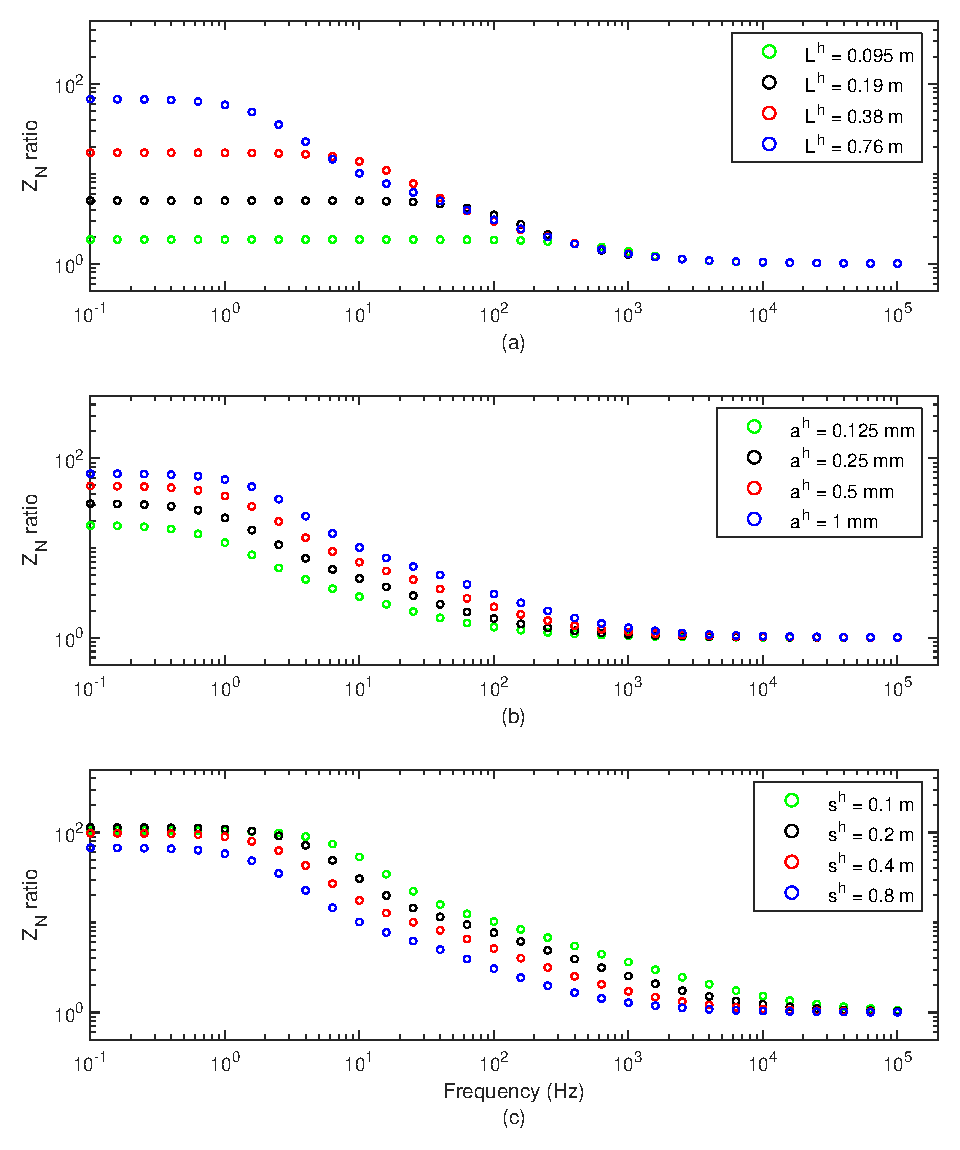
\includegraphics[ width=110mm, height=120mm]{sensitivityZN_geometry.eps}
\caption{
}
\label{fig.4}
\end{figure}

 \begin{figure}[!ht]
\centering
        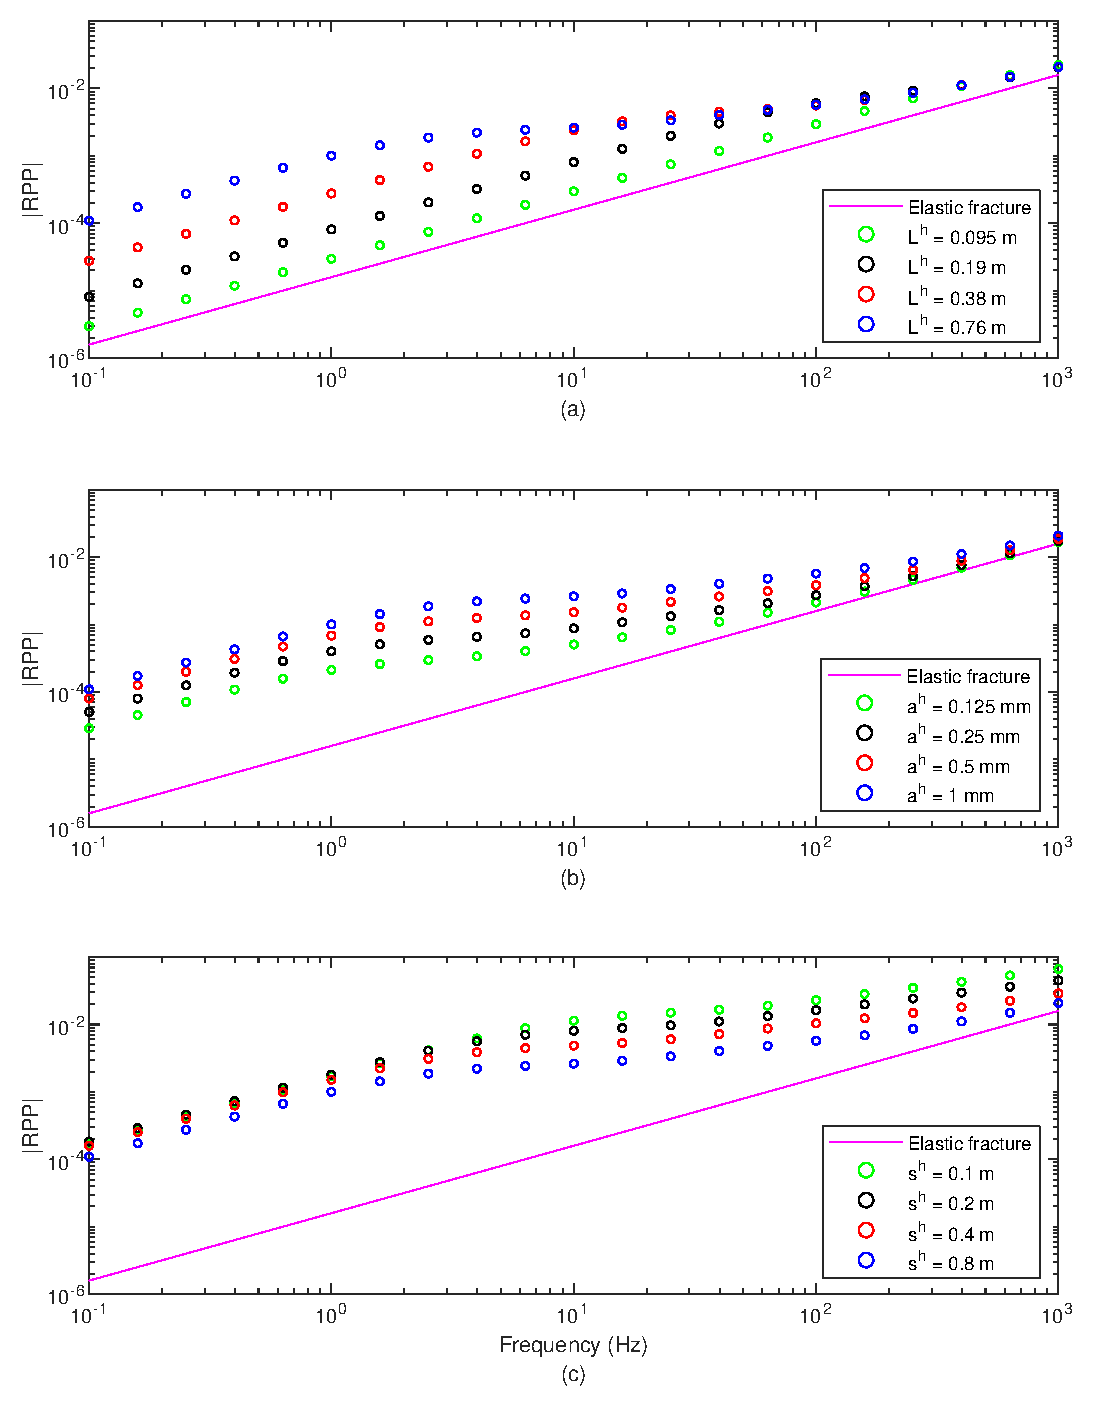
\includegraphics[ width=100mm, height=120mm]{sensitivityRPP_geometry.eps}
\caption{
}
\label{fig.5}
\end{figure}



\subsection{Sensitivity to the physical properties of the secondary fractures}
In this subsection, we investigate the sensitivity of the main fracture normal compliance and of its reflectivy response to the variation of physical  properties of the secondary fractures, such as their bulk $K_m^h$ and shear $\mu^h$ moduli, respectively, permeability $\kappa^h $ and fluid content $fluid^h$, respectively. To perform this sensitivity analysis, we modify one parameter at a time, taking as the reference values the ones specified in Table \ref{table.1}. For the case of the sensitivity to the mechanical moduli, we doubled the bulk modulus $K_m^h$ each time, keeping the ratio $K_m^h/ \mu^h =2$. To investigate the sensitivity to the permeability $\kappa^h$, we take increments in permeability of one order of magnitude from 0.1 D to 100 D. Finally, to study the sensitivity to the fluid content $fluid^f$, we compare the results of either considering water or gas as the saturating fluid of the secondary fractures.

 \begin{figure}[!ht]
\centering
        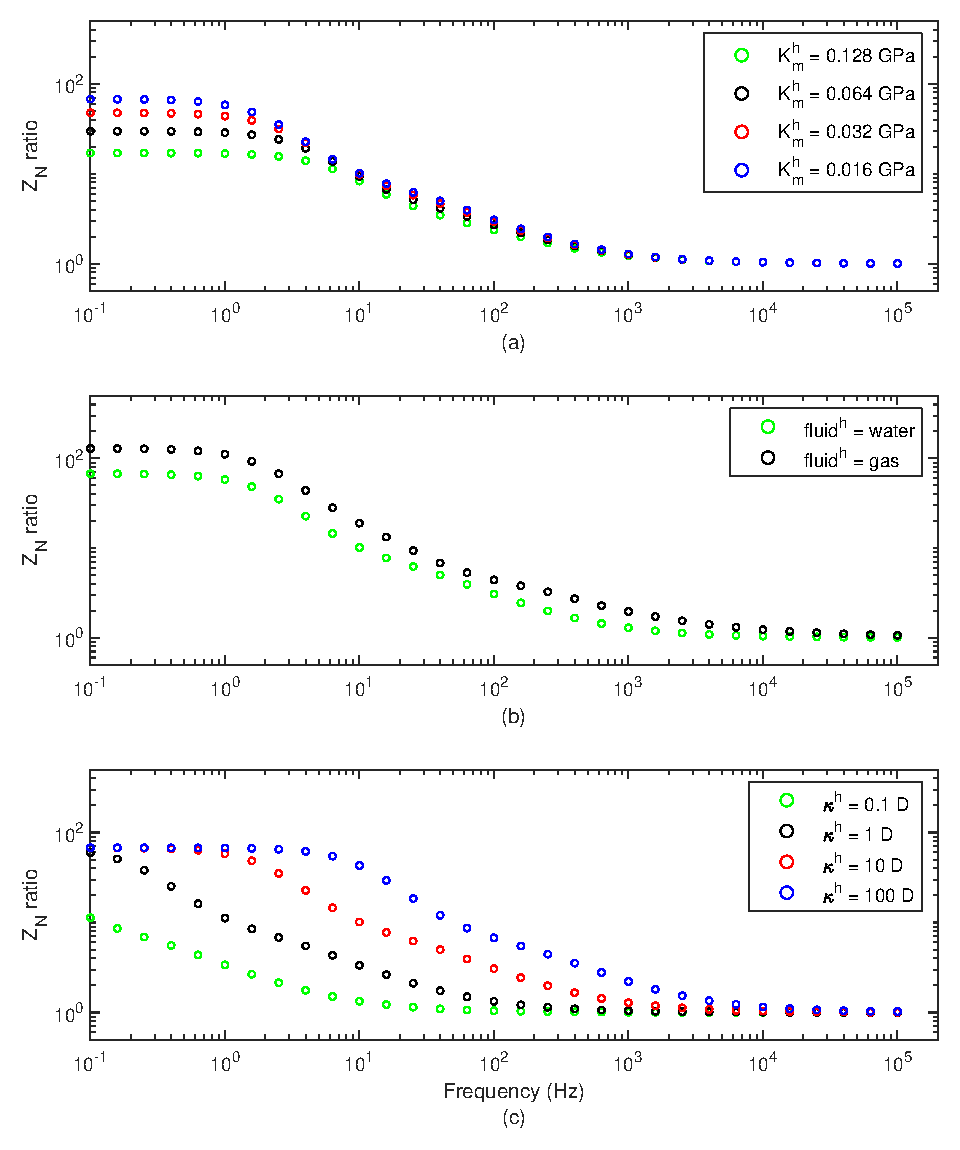
\includegraphics[ width=100mm, height=85mm]{sensitivityZN_physical.eps}
\caption{
}
\label{fig.6}
\end{figure}

 \begin{figure}[!ht]
\centering
        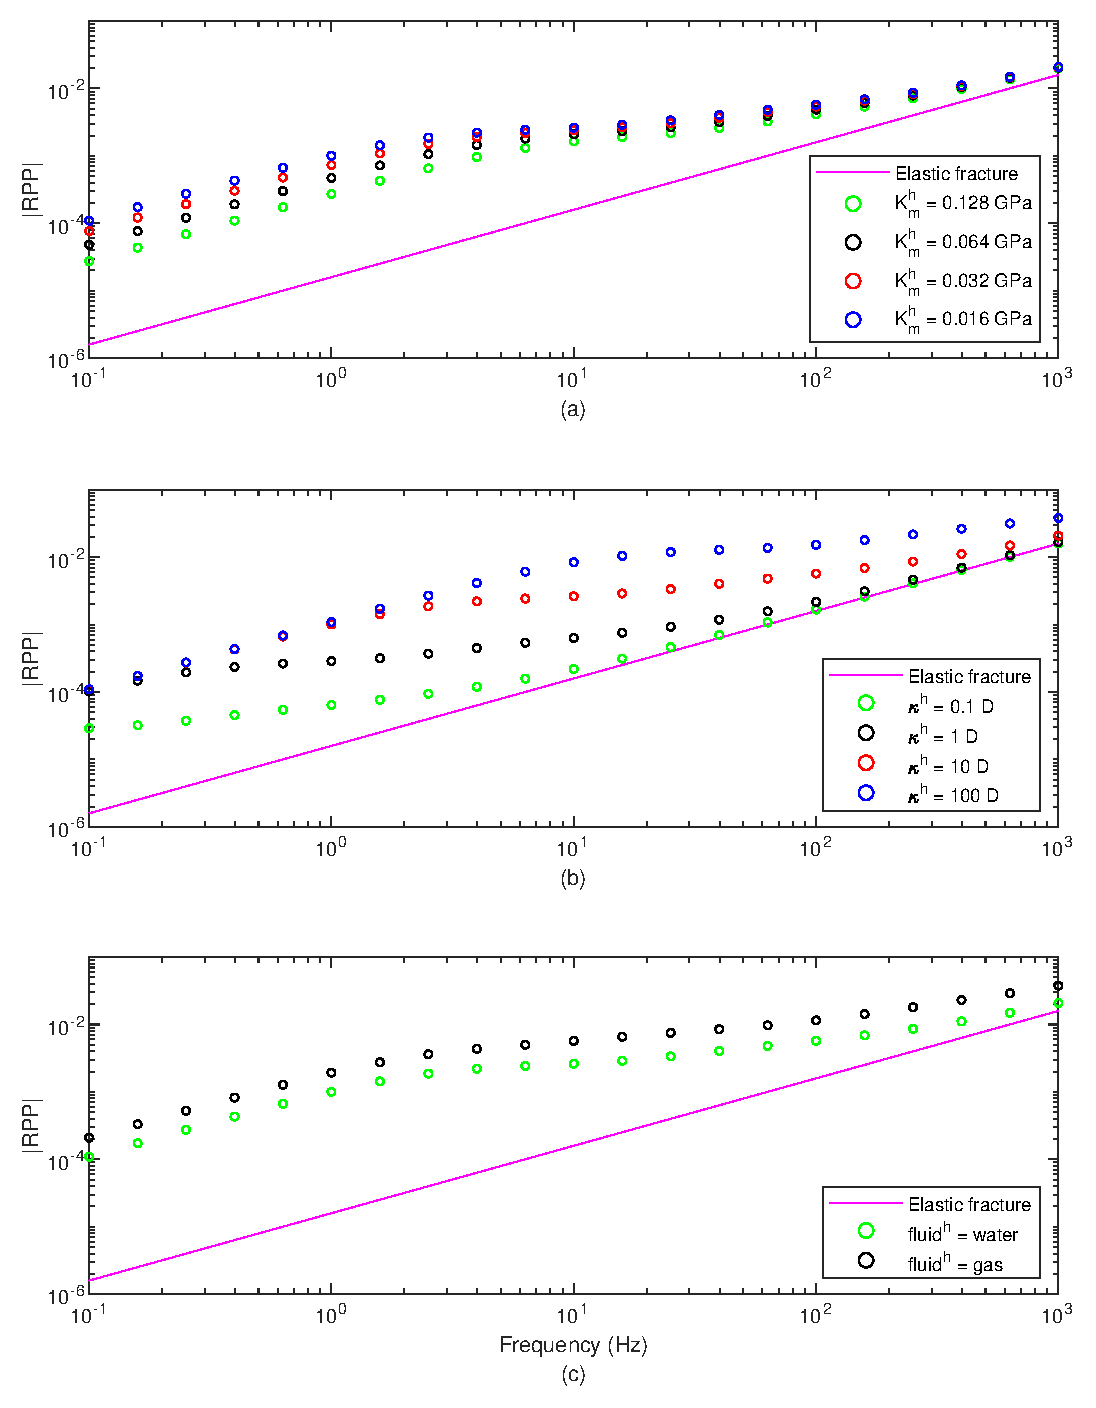
\includegraphics[ width=100mm, height=85mm]{sensitivityRPP_physical.eps}
\caption{
}
\label{fig.7}
\end{figure}

Figure \ref{fig.6}, presents the resulting $Z_N\, \text{ratio}$ as a function of frequency for the different physical parameters of the secondary fractures. As previously stated, these results also show that there is an overall increase of the normal compliance of the main fracture associated FPD with the secondary fractures for frequencies that are within the transition frequency and lower. Nonetheless, the sensitivity of the normal fracture compliance to variations of the tested physical properties present different outcomes. In this regard, the maximum  $Z_N\, \text{ratio}$ shows an increase 
of close to four-folds, from 17 to 67.5, corresponding to an eight-fold decrease in the bulk modulus $K_m^h$, from 0.128 GPa to 0.016 GPa (Figure \ref{fig.6}a). In contrast, the maximum  $Z_N\, \text{ratio}$ is not sensitive at all to variations in permeability, showing the same maximum value of 67.5 for all the tested permeabilities (Figure \ref{fig.6}b). We remark that for a permeability of 0.1 D, it is not possible to observe this maximum value because it occurs at a lower frequency than 0.1 Hz.
Finally, the maximum  $Z_N\, \text{ratio}$ increases close to two-folds, from 67.5 to 129.3, when considering gas instead of water as the saturating fluid in the secondary fractures (Figure \ref{fig.6}c). Regarding the sensitivity of the characteristic transition frequency $f_c$,  results show that $f_c$ increases from $\sim$ 6.3 Hz to $\sim$ 15.8 Hz as the bulk moduli $K_m^h$ increases. For the permeability $\kappa$, we disregard the first value of 0.1 D. Then, we observe that $f_c$ increases from $\sim$ 0.6 Hz to $\sim$  39.8 Hz as the permeability $\kappa^h$ increases. Finally, $f_c$ also increases from $\sim$ 6.3 Hz to $\sim$ 25.1 Hz when the saturating fluid $fluid^h$ changes from water to gas.


Next, \ref{fig.7} shows the corresponding sensitivity of the absolute value of PP reflectivities of the main fracture at normal incidence to the variations of the same parameters of the secondary fractures previously considered (Figure \ref{fig.6}). Overall, the results show that there is a maximum increase of the main fracture reflectivity of around two orders of magnitude with respect to its elastic value due to FPD with the secondary fractures. However, as already stated, its sensitivity to the tested physical 
properties of the secondary fractures is different. For an eight-fold decrease of bulk modulus $K_m^h$, the reflectivity shows a maximum increase of around one order of magnitude. In contrast, there are not changes of the maximum increase of reflectivity due to changes in permeability. Finally, considering gas instead of water as the saturating fluid produces an increase of reflectivity within the same order of magnitude.

\section{Discussion}
\subsection{sensitivities of the relaxed normal fracture compliance and  characteristic transition frequencies}
In this subsection we provide a general analysis about the effect of the geometrical and physical properties has on the of the main fracture normal compliance on its relaxed states and on the characteristic transition frequencies $f_c$. To this end, Figure \ref{fig.8} presents the $Z_N$ ratio corresponding to the FPD relaxed regime prevailing between the main and secondary fractures (relaxed $Z_N$ ratio)
with respect to the characteristic frequencies $f_c$ for every of the previous tested properties of the secondary fractures. The  $Z_N$ ratio in the relaxed  FPD state reflects the maximum increase that the normal fracture compliance can attain with respect to its undrained value for a given set of secondary fracture parameters (Figures \ref{fig.4} and  \ref{fig.6}).
These results show that, overall, the relaxed $Z_N ratio $ is the most sensitive to changes in the length $L^h$ of the secondary fractures, which presents a 35.6 fold increase for an eight fold increase of the length $L^h$.  This suggest that longer secondary fractures promote higher pressure gradients and provide greater pore volumes that enable the increase of the normal compliance of the main fracture as greater volumes of pore fluid flow towards the secondary fractures. Next, the changes in the bulk moduli $K_m^h$  and  in the aperture $a^h$  of the secondary fractures have similar impacts on the sensitivity of the relaxed  $Z_N$ ratio. This is, an eight fold decrease in the bulk modulus and a similar increase in the aperture produce around of a four fold increase in the corresponding relaxed $Z_N$ ratio, respectively. This implies that more deformable and wider secondary fractures can accommodate for more pore fluid from the main fracture as FPD takes place. Nonetheless, we remark that event though the changes in aperture reflect similar pore volume variations as those created by changes in the length, the corresponding relaxed $Z_N$ ratio sensitivity is much lower than that associated to the length of the secondary fractures. We suggest that this difference can be explained by the lower pressure gradients that variations in aperture produce in contrast to those induced by changes in length, which, in turn, results in a stiffer normal compliance of the main fracture as less fluid volume is drained to equilibrate its pore pressure with the secondary fractures. 
Then the spacing $s^h$ of the secondary fractures has a much lower impact than the aforementioned parameters on the sensitivity of the relaxed $Z_N$ ratio, where an eight-fold decrease of spacing produces close to a two-fold increase in the relaxed $Z_N$ ratio. Notice that decreasing spacing does not increase monotonically the relaxed $Z_N$ ratio. Specifically, the relaxed  $Z_N$ ratio increases with decreasing spacing achieving its maximum value for a spacing of 0.2 m then it decreases for the last tested value of spacing of 0.2 m. 


 \begin{figure}[!ht]
\centering
        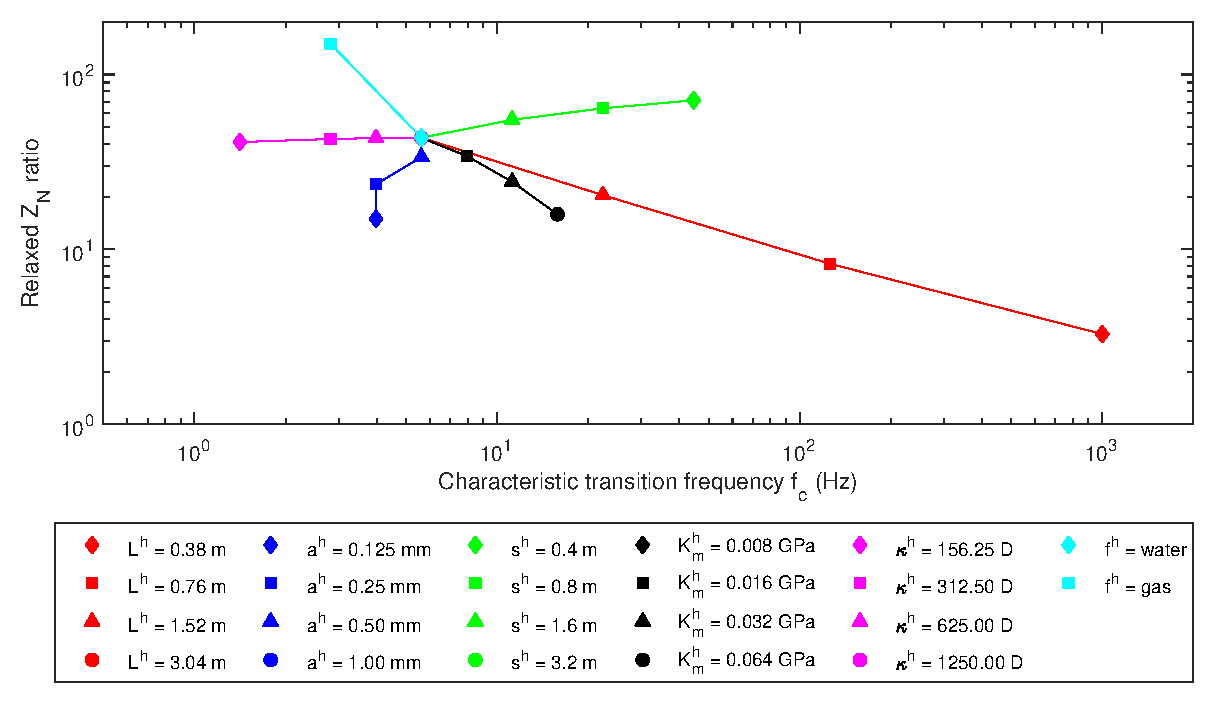
\includegraphics[ width=150mm, height=85mm]{sensitivity_summary.eps}
\caption{
}
\label{fig.8}
\end{figure}




\subsection{Effect of interconnected properties of the secondary fractures }
In the Results section we have tested the sensitivity of the compliance and reflectivity of the main fracture to the variation of several properties of the secondary fractures. For such case, the property of interest was modified at a time, while the 
others were kept constant. In contrast to the aforementioned analysis, in the following we assume that the properties of the secondary fractures are not independent but they are linked to their length directly or indirectly. This approach attempts to honor studies that show that the geometrical properties of fractures such their length and aperture are inter-related and that they can further be linked to their physical properties such as their permeability and bulk modulus. For our study, we use a power law  to relate the aperture $a^h$ to the length $L^h$ of the secondary fractures \cite<e.g.,>{Hatton1994}. This is $a^h = c_1 \, (L^h) ^{d_1}$, where $c_1$ = $10^{-2.9}$, $d_1$ = 1.49, respectively, which are values very similar to those suggested by \citeA{Hatton1994} for fractures with lengths smaller than 3 m. Likewise, we associate the permeability $\kappa^h$ of the secondary fractures to their hydraulic aperture $H^h$ through  the relationship \cite{Zimmerman1996,Jaeger2009}: $\kappa^h=(H^h)^2/12$, where the hydraulic aperture is related to the arithmetic mean aperture of the secondary fractures as \cite{Renshaw1995, Jaeger2009}: $(H^h)^3=(a^h)^3 ( 1 + r^2)^{-1.5}$. Here we assume that the  previously estimated aperture $a^h$ is the arithmetic mean aperture of the secondary fractures. Besides $r$ is the ratio between the corresponding standard deviation and the mean aperture, which we assume equal to 25. Similarly, it is also possible to relate the bulk $K_m^h$ and shear $\mu^h$ moduli of the secondary fractures to their drained normal $Z_N^h$ and tangential $Z_T^h$ compliances \cite{Nakagawa2007,Rubino2014}: $\mu^h = a^h/Z_T^h$ and $K_m^h =a^h/Z_N^h -4 \, a^h/(3\,Z_N^h)$, where the normal compliance of the secondary fractures can be further related to their length by a power law relationship  $Z_N^h = c_2 \, (L^h) ^{d_2}$, with $c_2$ = $10^{-10.8}$ and $d_2$ =0.77, respectively. This specific curve follows the trend of the data presented in \citeA{Barbosa2019}. Notice that the relationships for estimating the aperture and permeability of the secondary fractures show a monotonically increasing trend with respect to their length and aperture, respectively. The relationships to estimate the respective shear and bulk moduli have a similar behavior but no with respect to a single variable but with respect to the ratio  of the aperture to the tangential and drained normal compliance. Consequently, the moduli are related to the aperture and the compliances in an opposing fashion.
Table \ref{table.3} summarizes the geometrical and physical properties found after considering three different secondary fracture lengths: 0.19 m, 0.38 m and 0.76 m, respectively. Other properties are assumed to be the same for all cases and correspond to those listed in Table \ref{table.1}.  As expected, the estimated apertures and permeabilities of the secondary fractures increase with their length. A similar behavior is observed for the bulk and shear moduli, but, as explained, their increase correlates to the ratio of the aperture to the respective tangential and drained normal compliance.  For reference,  Table \ref{table.3} also presents the estimated normal and tangential compliance of the secondary fractures, which show an increasing compliant behavior with increasing length of the secondary fractures increases. Besides, we assume that both the main and secondary fractures are water saturated, where the properties of the water are those presented in Table \ref{table.2}.


\begin{table}[!ht]
  \caption{ Properties of the secondary fractures related to their length }
\begin{center}
  \begin{tabular}{ | l c  c  c | }
    \hline
    Property  & \multicolumn{3}{c |}{Secondary fracture ($h$)} \\ 
    \hline
    Length $L$ (m) & 0.19 & 0.38 & 0.76  \\
    Aperture $a$ (m) & 1.e-4 & 3.e-4 & 8.e-4\\
    Permeability $\kappa$ (D) & 1.5 & 12.0 & 94.4\\
    Frame bulk modulus $K_m$ (GPa)  & 0.013 & 0.021 & 0.035 \\ 
    Frame shear modulus $\mu$ (GPa) & 0.0084 & 0.014 & 0.023\\
    Normal compliance $Z_N$ (m/Pa)  & 4.4e.-12 & 7.5e-12 & 1.3e-11 \\
    Tangential compliace $Z_T$ (m/Pa) & 1.3e-11 & 2.1e-11 & 3.7e-11 \\
    
    \hline
  \end{tabular}
  \label{table.3}
\end{center}
\end{table}

Figure \ref{fig.9} shows the impact that the three different sets of properties of the secondary fractures (Table \ref{table.3}) has on the  main fracture normal compliance (Figure \ref{fig.8}a) and on the corresponding PP reflectivity (Figure \ref{fig.9}a) at normal incidence, respectively. Regarding effects on the main fracture compliance, Figure \ref{fig.9}a shows that the maximum $Z_N ratio$ takes increasingly higher values of  2.6, 9.2 and 36.4 as the length $L^h$ of the secondary fractures increases. This behavior suggest that, for this example, it is the length of the secondary fractures that controls the FPD process, as longer secondary fractures generate higher pressure gradients and provide greater pore volumes that permit the drainage of higher volumes of the saturating fluid from the main fracture, which in turn, increases the main fracture normal compliance. This further implies that this process dominates the opposite tendency that the higher stiffness of longer secondary fractures induces (Figure \ref{fig.7}a). Regarding, the transition frequency $f_c$, we observe a dominance of the effect of the  higher permeability of longer secondary fractures, since it promotes an increase of $f_c$ , which is similar to the effect observed in Figure \ref{fig.7}b. This outcome further implies that the tendency of that longer secondary fractures to decrease $f_c$ (Figure \ref{fig.6}a) is, for this example, 


 \begin{figure}[!ht]
\centering
        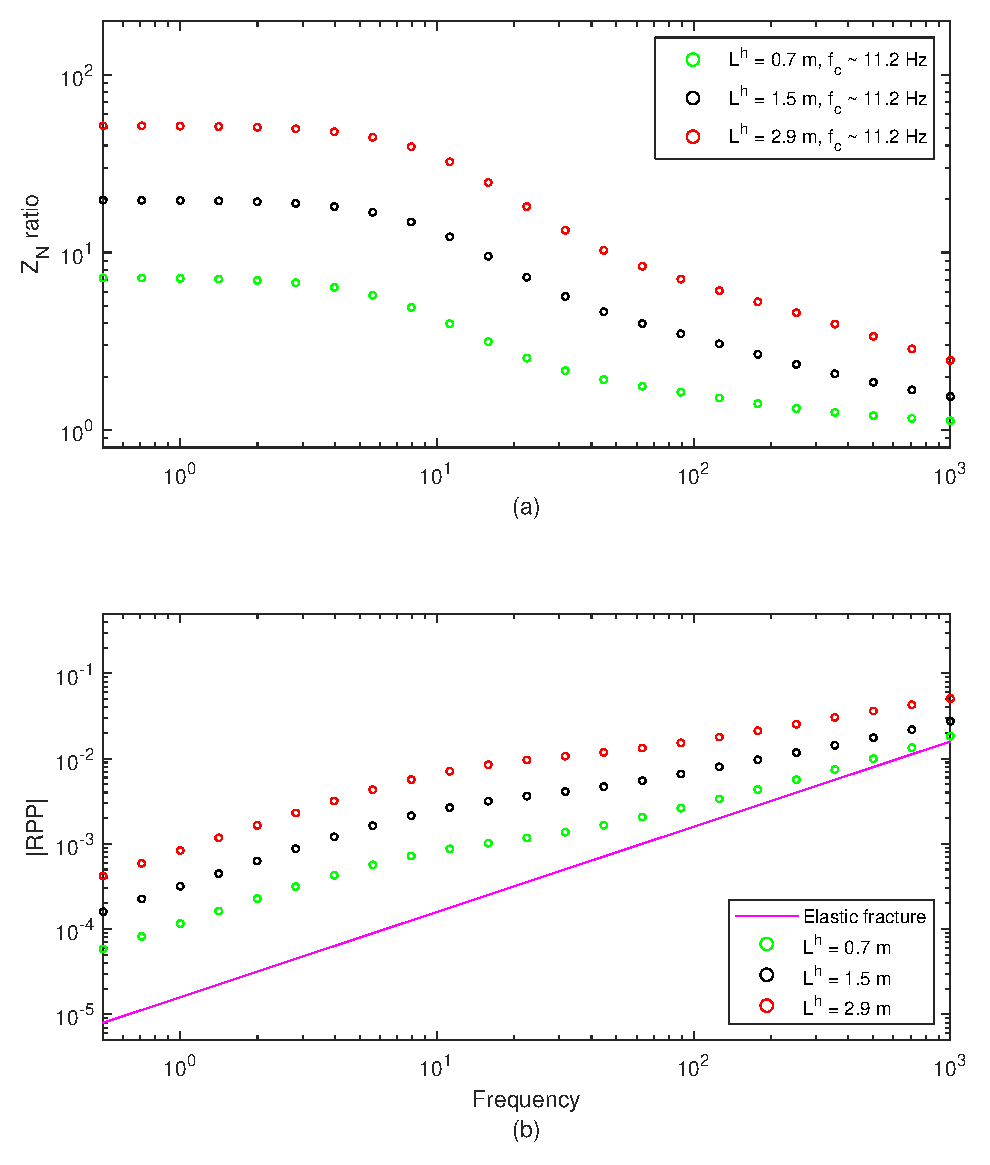
\includegraphics[ width=100mm, height=85mm]{linkedProperties.eps}
\caption{
}
\label{fig.9}
\end{figure}

\section{Conclusions}

%Text here ===>>>

%  To add line numbers to lines in equations,
%  \begin{linenomath*}
%  \begin{equation}
%  \end{equation}
%  \end{linenomath*}



%% Enter Figures and Tables near as possible to where they are first mentioned:
%
% DO NOT USE \psfrag or \subfigure commands.
%
% Figure captions go below the figure.
% Table titles go above tables;  other caption information
%  should be placed in last line of the table, using
% \multicolumn2l{$^a$ This is a table note.}
%
%----------------
% EXAMPLE FIGURES
%
% \begin{figure}
% \includegraphics{example.png}
% \caption{caption}
% \end{figure}
%
% Giving latex a width will help it to scale the figure properly. A simple trick is to use \textwidth. Try this if large figures run off the side of the page.
% \begin{figure}
% \noindent\includegraphics[width=\textwidth]{anothersample.png}
%\caption{caption}
%\label{pngfiguresample}
%\end{figure}
%
%
% If you get an error about an unknown bounding box, try specifying the width and height of the figure with the natwidth and natheight options. This is common when trying to add a PDF figure without pdflatex.
% \begin{figure}
% \noindent\includegraphics[natwidth=800px,natheight=600px]{samplefigure.pdf}
%\caption{caption}
%\label{pdffiguresample}
%\end{figure}
%
%
% PDFLatex does not seem to be able to process EPS figures. You may want to try the epstopdf package.
%

%
% ---------------
% EXAMPLE TABLE
% Please do NOT include vertical lines in tables
% if the paper is accepted, Wiley will replace vertical lines with white space
% the CLS file modifies table padding and vertical lines may not display well
%

%% SIDEWAYS FIGURE and TABLE
% AGU prefers the use of {sidewaystable} over {landscapetable} as it causes fewer problems.
%
% \begin{sidewaysfigure}
% \includegraphics[width=20pc]{figsamp}
% \caption{caption here}
% \label{newfig}
% \end{sidewaysfigure}
%
%  \begin{sidewaystable}
%  \caption{Caption here}
% \label{tab:signif_gap_clos}
%  \begin{tabular}{ccc}
% one&two&three\\
% four&five&six
%  \end{tabular}
%  \end{sidewaystable}

%% If using numbered lines, please surround equations with \begin{linenomath*}...\end{linenomath*}
%\begin{linenomath*}
%\begin{equation}
%y|{f} \sim g(m, \sigma),
%\end{equation}
%\end{linenomath*}

%%% End of body of article

%%%%%%%%%%%%%%%%%%%%%%%%%%%%%%%%
%% Optional Appendix goes here
%
% The \appendix command resets counters and redefines section heads
%
% After typing \appendix
%
%\section{Here Is Appendix Title}
% will show
% A: Here Is Appendix Title
%
\appendix
\section{Here is a sample appendix}

%%%%%%%%%%%%%%%%%%%%%%%%%%%%%%%%%%%%%%%%%%%%%%%%%%%%%%%%%%%%%%%%
%
% Optional Glossary, Notation or Acronym section goes here:
%
%%%%%%%%%%%%%%
% Glossary is only allowed in Reviews of Geophysics
%  \begin{glossary}
%  \term{Term}
%   Term Definition here
%  \term{Term}
%   Term Definition here
%  \term{Term}
%   Term Definition here
%  \end{glossary}

%
%%%%%%%%%%%%%%
% Acronyms
%   \begin{acronyms}
%   \acro{Acronym}
%   Definition here
%   \acro{EMOS}
%   Ensemble model output statistics
%   \acro{ECMWF}
%   Centre for Medium-Range Weather Forecasts
%   \end{acronyms}

%
%%%%%%%%%%%%%%
% Notation
%   \begin{notation}
%   \notation{$a+b$} Notation Definition here
%   \notation{$e=mc^2$}
%   Equation in German-born physicist Albert Einstein's theory of special
%  relativity that showed that the increased relativistic mass ($m$) of a
%  body comes from the energy of motion of the body—that is, its kinetic
%  energy ($E$)—divided by the speed of light squared ($c^2$).
%   \end{notation}



\section{Open Research}
AGU requires an Availability Statement for the underlying data needed to understand, evaluate, and build upon the reported research at the time of peer review and publication.

Authors should include an Availability Statement for the software that has a significant impact on the research. Details and templates are in the Availability Statement section of the Data and Software for Authors Guidance: \url{https://www.agu.org/Publish-with-AGU/Publish/Author-Resources/Data-and-Software-for-Authors#availability}

It is important to cite individual datasets in this section and, and they must be included in your bibliography. Please use the type field in your bibtex file to specify the type of data cited. Some options include Dataset, Software, Collection, ComputationalNotebook. Ex: 
\\
\begin{verbatim}

@misc{https://doi.org/10.7283/633e-1497,
  doi = {10.7283/633E-1497},
  url = {https://www.unavco.org/data/doi/10.7283/633E-1497},
  author = {de Zeeuw-van Dalfsen, Elske and Sleeman, Reinoud},
  title = {KNMI Dutch Antilles GPS Network - SAB1-St_Johns_Saba_NA P.S.},
  publisher = {UNAVCO, Inc.},
  year = {2019},
  type = {dataset}
}

\end{verbatim}

For physical samples, use the IGSN persistent identifier, see the International Geo Sample Numbers section:
\url{https://www.agu.org/Publish-with-AGU/Publish/Author-Resources/Data-and-Software-for-Authors#IGSN}
%%%%%%%%%%%%%%%%%%%%%%%%%%%%%%%%%%%%%%%%%%%%%%%

\acknowledgments
This section is optional. Include any Acknowledgments here.



%% ------------------------------------------------------------------------ %%
%% References and Citations

%%%%%%%%%%%%%%%%%%%%%%%%%%%%%%%%%%%%%%%%%%%%%%%
%
% \bibliography{<name of your .bib file>} don't specify the file extension
%
% don't specify bibliographystyle

% In the References section, cite the data/software described in the Availability Statement (this includes primary and processed data used for your research). For details on data/software citation as well as examples, see the Data & Software Citation section of the Data & Software for Authors guidance
% https://www.agu.org/Publish-with-AGU/Publish/Author-Resources/Data-and-Software-for-Authors#citation

%%%%%%%%%%%%%%%%%%%%%%%%%%%%%%%%%%%%%%%%%%%%%%%

\bibliography{reference}



%Reference citation instructions and examples:
%
% Please use ONLY \cite and \citeA for reference citations.
% \cite for parenthetical references
% ...as shown in recent studies (Simpson et al., 2019)
% \citeA for in-text citations
% ...Simpson et al. (2019) have shown...
%
%
%...as shown by \citeA{jskilby}.
%...as shown by \citeA{lewin76}, \citeA{carson86}, \citeA{bartoldy02}, and \citeA{rinaldi03}.
%...has been shown \cite{jskilbye}.
%...has been shown \cite{lewin76,carson86,bartoldy02,rinaldi03}.
%... \cite <i.e.>[]{lewin76,carson86,bartoldy02,rinaldi03}.
%...has been shown by \cite <e.g.,>[and others]{lewin76}.
%
% apacite uses < > for prenotes and [ ] for postnotes
% DO NOT use other cite commands (e.g., \citet, \citep, \citeyear, \citealp, etc.).
% \nocite is okay to use to add references from your Supporting Information
%



\end{document}



More Information and Advice:

%% ------------------------------------------------------------------------ %%
%
%  SECTION HEADS
%
%% ------------------------------------------------------------------------ %%

% Capitalize the first letter of each word (except for
% prepositions, conjunctions, and articles that are
% three or fewer letters).

% AGU follows standard outline style; therefore, there cannot be a section 1 without
% a section 2, or a section 2.3.1 without a section 2.3.2.
% Please make sure your section numbers are balanced.
% ---------------
% Level 1 head
%
% Use the \section{} command to identify level 1 heads;
% type the appropriate head wording between the curly
% brackets, as shown below.
%
%An example:
%\section{Level 1 Head: Introduction}
%
% ---------------
% Level 2 head
%
% Use the \subsection{} command to identify level 2 heads.
%An example:
%\subsection{Level 2 Head}
%
% ---------------
% Level 3 head
%
% Use the \subsubsection{} command to identify level 3 heads
%An example:
%\subsubsection{Level 3 Head}
%
%---------------
% Level 4 head
%
% Use the \subsubsubsection{} command to identify level 3 heads
% An example:
%\subsubsubsection{Level 4 Head} An example.
%
%% ------------------------------------------------------------------------ %%
%
%  IN-TEXT LISTS
%
%% ------------------------------------------------------------------------ %%
%
% Do not use bulleted lists; enumerated lists are okay.
% \begin{enumerate}
% \item
% \item
% \item
% \end{enumerate}
%
%% ------------------------------------------------------------------------ %%
%
%  EQUATIONS
%
%% ------------------------------------------------------------------------ %%

% Single-line equations are centered.
% Equation arrays will appear left-aligned.

Math coded inside display math mode \[ ...\]
 will not be numbered, e.g.,:
 \[ x^2=y^2 + z^2\]

 Math coded inside \begin{equation} and \end{equation} will
 be automatically numbered, e.g.,:
 \begin{equation}
 x^2=y^2 + z^2
 \end{equation}


% To create multiline equations, use the
% \begin{eqnarray} and \end{eqnarray} environment
% as demonstrated below.
\begin{eqnarray}
  x_{1} & = & (x - x_{0}) \cos \Theta \nonumber \\
        && + (y - y_{0}) \sin \Theta  \nonumber \\
  y_{1} & = & -(x - x_{0}) \sin \Theta \nonumber \\
        && + (y - y_{0}) \cos \Theta.
\end{eqnarray}

%If you don't want an equation number, use the star form:
%\begin{eqnarray*}...\end{eqnarray*}

% Break each line at a sign of operation
% (+, -, etc.) if possible, with the sign of operation
% on the new line.

% Indent second and subsequent lines to align with
% the first character following the equal sign on the
% first line.

% Use an \hspace{} command to insert horizontal space
% into your equation if necessary. Place an appropriate
% unit of measure between the curly braces, e.g.
% \hspace{1in}; you may have to experiment to achieve
% the correct amount of space.


%% ------------------------------------------------------------------------ %%
%
%  EQUATION NUMBERING: COUNTER
%
%% ------------------------------------------------------------------------ %%

% You may change equation numbering by resetting
% the equation counter or by explicitly numbering
% an equation.

% To explicitly number an equation, type \eqnum{}
% (with the desired number between the brackets)
% after the \begin{equation} or \begin{eqnarray}
% command.  The \eqnum{} command will affect only
% the equation it appears with; LaTeX will number
% any equations appearing later in the manuscript
% according to the equation counter.
%

% If you have a multiline equation that needs only
% one equation number, use a \nonumber command in
% front of the double backslashes (\\) as shown in
% the multiline equation above.

% If you are using line numbers, remember to surround
% equations with \begin{linenomath*}...\end{linenomath*}

%  To add line numbers to lines in equations:
%  \begin{linenomath*}
%  \begin{equation}
%  \end{equation}
%  \end{linenomath*}



